%\documentclass[xcolor=dvipsnames]{beamer}
\documentclass[8pt]{beamer}
\usetheme{Madrid}
\usepackage{color, colortbl, xcolor}
\definecolor{UBCblue}{rgb}{0.94706, 0.13725, 0.26667}
\usecolortheme[named=UBCblue]{structure}
\usepackage{amsfonts}


\useoutertheme[right, width= 0.125\paperwidth]{sidebar}


\usepackage{tikz-cd}


%math symbols
\usepackage{graphicx, amsmath, amssymb, longtable, mathtools, amsthm, polynom, mathrsfs, cancel}
%\usepackage{enumitem}

%\newcommand{\tabitem}{~~\llap{\textbullet}~~}
\newcommand{\tabitem}{\textbullet~}
\usepackage{url}
\usepackage{breakcites}
\usepackage{comment}
\usepackage[table]{xcolor}
\usepackage{booktabs} % Optional: for better looking horizontal lines

%Bibtex
\usepackage[backend=biber,style=alphabetic]{biblatex}
\addbibresource{references.bib}
%\usepackage[breaklinks]{hyperref}
%\appto\bibfont{\setlength{\emergencystretch}{.1em}}


%Theorem Like Environments

%\newtheorem{theorem}{Theorem} 
%\numberwithin{theorem}{section}




%\newtheorem{definition}{Definition}
%\numberwithin{definition}{section}

\newtheorem{assumption}{Assumption}
\numberwithin{assumption}{section}

%\newtheorem{proposition}{Proposition}
%\numberwithin{proposition}{section}

%\newtheorem{remark}{Remark}
%\numberwithin{remark}{section}

%\newtheorem{corollary}{Corollary}
%\numberwithin{corollary}{section}

%\newtheorem{conjecture}{Conjecture}
%\numberwithin{conjecture}{section}

%\newtheorem{example}{Example}
%\numberwithin{example}{section}


%\usepackage{comment}
%\renewenvironment{comment}{}{}
\usepackage{algorithm}
\usepackage{algpseudocode} 
%\usepackage{algorithm2e}

%Tabular packages
\usepackage{multicol, multirow, array, tabularx, caption, float}
\newcolumntype{C}[1]{>{\centering\arraybackslash}p{#1}}
%Tikz package
\usepackage{tikz}
\usetikzlibrary{positioning}
\usepackage{subcaption}

%set margins



%Common sets and symbols:
\newcommand{\R}{\mathbb{R}}
\newcommand{\Z}{\mathbb{Z}}
\newcommand{\N}{\mathbb{N}}
\newcommand{\Q}{\mathbb{Q}}
\newcommand{\C}{\mathbb{C}}
\newcommand{\F}{\mathbb{F}}
\newcommand{\bigS}{\mathcal{S}}

\newcommand{\Open}{\mathcal{O}}
\newcommand{\E}{\mathbb{E}}
\newcommand{\I}{\mathbb{I}}
\newcommand{\Var}{\mathbf{Var}}
\newcommand{\bset}[1]{\left \lbrace #1 \right \rbrace}
\newcommand{\aset}[1]{\left \langle #1 \right \rangle}
\newcommand{\mexists}{\; \exists \;}
\newcommand{\mforall}{\; \forall \;}
\newcommand{\cunion}[2]{\bigcup_{#1 = #2}^\infty}
\newcommand{\cinter}[2]{\bigcap_{#1 = #2}^\infty}
\newcommand{\csum}[2]{\sum_{#1 = #2}^\infty}
\newcommand{\dist}{\mathrm{dist}}
\newcommand{\Span}[1]{\mathrm{Span}\bset{#1}}
\newcommand{\id}{\mathrm{id}}
\newcommand{\im}{\mathrm{im}}
\newcommand{\D}{\displaystyle}
\newcommand{\Cov}{\mathrm{Cov}} 
\newcommand{\intp}[1] {\D \int_\Omega {#1 } \; d \mathbb P}
\newcommand{\HS}{\mathrm{HS}}

\newcommand{\NT}[2]{N_\mathbf{#1}^{\text{#2}}}
\newcommand{\T}[2]{\mathcal T_\mathbf{#1}^{\text{#2}}}

\newcommand{\bA}{\mathbf A}
\newcommand{\bB}{\mathbf B}
\newcommand{\CH}{\mathcal H}
\newcommand{\Mres}{M_\text{res}}
%\renewenvironment{comment}{}{}

\newcommand{\globalLGheight}{0.23\textheight}
\newcommand{\globalLGwidth}{0.87\textwidth}

\title{Option Pricing For Weather-Based Derivatives}
\author{Trajan Murphy}
\date{\today}

\begin{document}
	
	\maketitle


\begin{frame}{Motivation}
	\begin{block}{Goal:}
		Model call/put options based on weather for weather-sensitive industries
		
		
		\end{block}
	
\begin{figure}[h!]
	\centering
	\begin{subfigure}[b]{0.3\textwidth}
		
\includegraphics[width=0.9\textwidth,height = 0.2\textheight]{Air Travel.jpg}
		\caption*{Air Travel}
	
	\end{subfigure}
	\hfill
	\begin{subfigure}[b]{0.3\textwidth}
		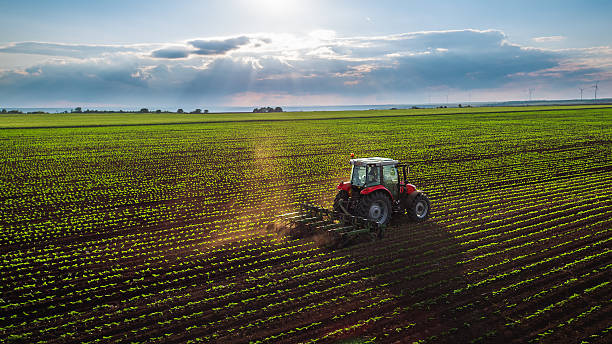
\includegraphics[width=0.9\textwidth,height = 0.2\textheight]{Agriculture.jpg}
		\caption*{Agriculture}

	\end{subfigure}
	\hfill
	\begin{subfigure}[b]{0.3\textwidth}
		
\includegraphics[width=0.9\textwidth,height = 0.2\textheight]{Tourism.jpg}
		\caption*{Tourism}
		\label{TTou}
	\end{subfigure}
\end{figure}


\end{frame}

\begin{frame}{Ornstein–Uhlenbeck Process \cite{gibert2024monte}}
	 Gauss-Markov process defined by SPDE:
	\begin{block}{Mean-reverting OU-Process}
		$$dT_t = \kappa(\overline T_t - T_t)dt + \sigma_t dW_t$$
	\end{block}
	
	\begin{itemize}
		\item $T_t$ = Daily average temperature at time $t$
		\item $\overline T_t$ = mean temperature at time $t$
		\item $\kappa$ = ``constant"
		\item $\sigma_t$ = volatility at time $t$
		\item $W_t$ = Wiener process
	\end{itemize}
	
	\begin{block}{Explicit Solution}
		$$T_t = \overline T_t + \exp \left( -\int_0^t \kappa du \right) \int_0^t \exp \left( \int_0^t \kappa du \right) \sigma_t dW_t $$
	\end{block}
\end{frame}

\begin{frame}{Call/Put Pricing \cite{gibert2024monte}}
	Degree Days (Heating/Cooling)
	\begin{itemize}
		\item $CDD_n = (T_n - 65)^+, \qquad n \in \text{Nov 15, ..., Mar 15}$
		\item $HDD_n = (65 - T_n)^+, \qquad n \in \text{May 15, ..., Oct 15}$
		\item $DD_N = \sum_{n =1}^N CDD_n $ (or $HDD_n$)
	
	\end{itemize}
	
	\vspace{10pt} 
	
	Let $K_c$ = strike price, $\alpha$ = payout rate, $C$ = cap price. Then 
	\begin{itemize}
		\item Call price = $\min \bset{\alpha(DD - K_c)^+, C}$
		\item Put price = $\min \bset{\alpha(K_c - D)^+, C}$
	\end{itemize}
	
	\vspace{10pt}
	
	Typical values are $2.5K \leq \alpha \leq 5K$, $0.5M \leq C \leq 1M$
	
	
	
\end{frame}


\begin{frame}{Application}
	\begin{enumerate}
		\item Use hourly dry bulb temperature from Boston Logan Airport in 2012
		\cite{NCEI2026}
		\item Estimate daily average using trapezoidal integration
		\item Fit daily average temperature with quadratic regression 
		\item Compute ACF and PACF of residuals
		\item Estimate $\sigma_t$ by using a monthly average and linearly interpolate to get daily values
		\item Estimate $T_t$ using OH equation with $\kappa \equiv 1$
		\item Compute call and put options based on modeled temperature
		\item Run MC simulations 
	\end{enumerate}
\end{frame}

\begin{frame}{References}
	\printbibliography
\end{frame}
\end{document}